\chapter{The standard model}

\label{ch:sm}

\section{Introduction}
\par What're the most fundamental particles that constitute our world? How do the particles interact with each other? These are the two most essential questions people are trying to explain for centuries.

\par By the early twentieth century, scientists believed that atoms were the building blocks of nature. People trusted Newtonian laws of motion which solved most problems of physics.

\par The establishment of Einstein's theory of relativity and a growing field of quantum mechanics then 
challenged the fundamental precepts of physics at that time. Just as Max Born predicted ``Physics as we know it will be over in six months''.

\par Guided by both theoretical models and experimental discoveries, the well-developed Quantum field theory became very successful in describing particles as well as 
interactions between them (electromagnetic and weak interaction). Subatomic particles were then revealed: neutron (1931), muon (1937), pions (1947), kaons (1949), and eventually, the eruption of discoveries of mesons and baryons in the 1950s and 1960s, called ``particle zoo''.

\par Starting from 1964 when Murray Gell-Mann and George Zweig put forth the idea of quarks, the standard model is gradually completed and finally summarized by John Iliopoulos in 1974.

\par In section 2.2 and 2.3, a overview of the standard model particle physics and their interactions are given, while
a brief description of gauge theory is in section 2.4. We introduced the formation of Lagrangian of the SM in section 2.5 to expain the how particles gain their masses via Higgs mechanism in section 2.5.

\section{Particles}
% Standard model particle table
\begin{figure}[htbp]
  \begin{center}
    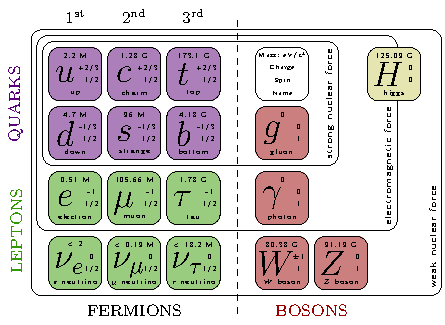
\includegraphics[width=0.8\textwidth]{chapters/c1/figures/sm-particle-table}
  \end{center}
  \caption{Particles of the Standard Model of particle physics}
  \label{fig:c1smparticletable}
\end{figure}
\par Demonstrated in Fig~\ref{fig:c1smparticletable}, the fundamental building blocks of matter are fermions with half-integer spin in the SM, while the mediators of forces of their interactions are gauge fermion bosons with integer spin. The spin-0 scalar Higgs boson is the origin of the mass of other particles.

\begin{itemize}
  \item \textbf{Fermions} could be divided into two categories: quarks, and leptons. There are three generations of both kinds: the first generation made up common matter, and the higer generations can be accessed at higher energies.
  \item \textbf{Quarks} Each generation of quarks have two types: up-type with a charge of $\frac{2}{3}$ and down-type with a charge of -$\frac{1}{3}$ and both could interact through electromagnetic force. The color charge carried by quarks makes them able to 
interact via strong interaction. Asymptotic freedom explains why quarks need to bind with together, resulting in the color-neutral particles called \textit{hadrons}. There are two types of hadrons: \textit{baryons} and \textit{mesons}. Protons and neutrons are two examples of baryons while pion and kaon are examples of mesons. Weak isospin makes quarks able to couple via weak interaction like fermions.
  \item \textbf{Leptons} Each generation has a charged particle and a electrically neutral neutrino. Leptons don't have color charge so that they can't interact via strong iteration. While the charged particle could interact through electromagnetic and weak force as they has both charge and weak isospin, the electrically neutral neutrinos could only interact via weak interaction, making them extremely hard to be detected in experiments.
  \item \textbf{Bosons} as mediators for the three types of force in the standard model listed below.
  \item \textbf{Photon} which is discovered very early, is the mediator of the electromagnetic force. It's a massless, electromagnetic-charge-neutral, spin-1 particle.
  \item \textbf{Gluon} is first discovered at DESY in the late 1970s and is the mediator of the strong force. Gluons are massless, spin-1 particles. The gluon caries color charge itself and could interact quarks. There are eight varieties of gluons as there are nine different combinations of the color charge in which the singlet state $\frac{r\bar{r}+b\bar{b}+g\bar{g}}{\sqrt{3}}$ does not exist.
\end{itemize}

\par The \textbf{$W^{\pm}$} and \textbf{Z} bosons are discovered at the UA1 and UA2 experiments in the late 1980s and serve as mediators of the weak force. They are spin-1 particles with masses around 80 and 91 GeV. The \textbf{$W^{\pm}$} bosons carry both the weak charged current and electromagnetic charges of ±1, while the Z boson is the mediator of the weak neutral current and electromagnetic-charge-neutral. \textbf{Higgs} boson is discovered at the CMS and ATLAS experiments in 2012. Higgs is a spin-0 scalar neutral particle with mass. Fermions and bosons acquired their mass through Yukawa coupling with the Higgs field. 

\section{Interactions}
\begin{table}[tbh]
\centering
\tiny
\begin{tabular}{|l|c|c|c|c|c|c}
\hline
    Force typle & Mediator & Affected particles & Acts on & Coupling& Scale of magnitude\\
    &&&&Constant &at the scale of quarks\\
    &&&&& (relative to electromagnetism)\\
\hline
\hline
    Electromagnetic  & $\gamma$&Electrically charged fermions&Electric charge& $\alpha$ &$1$\\
    Strong [years] & $g$ &Quarks, glouns & Color charge& $\alpha_s$ &$60$\\
    Weak & $W^{\pm}, Z$ &Left-handed fermions & Flavor& $\alpha_W$ &$10^{-4}$\\
\hline

\end{tabular}
\caption{Coupling constants of the three Standard Model forces. }
\label{tab:forces}
\end{table}

\par Table ~\ref{tab:forces} summarized relevant values of the three different interaction vertices including the values of coupling constants at low energy. At low energies, the weak force is actually much weaker than the electromagnetic force at low energies, even though the weak coupling constant is relatively larger. This is because the strength of weak interactions is suppressed by the large masses the W and Z bosons. The weak force becomes stronger than the electromagnetic force as values of coupling constants change.

\section{Gauge theory}
\par Gauge Theory is a type of field theory in which the Lagrangian is invariant under certain Lie groups of local transformations. As a gauge theory, the SM Lagrangian is under transformations of the group $SU(3)_c \times SU(2)_L \times U(1)_Y$.

\par The matter content of the SM is described by representations of the symmetry group, while the local gauge symmetry is represented by a force mediated by gauge bosons.

\par There are twelve gauge bosons in total: eight gluons which correspond to the generators of $SU(3)_c$, $W^{\pm}$ bosons which correspond to generators of $SU(2)_L$, and the Z boson and $\gamma$ which correspond to linear combinations of generators for $SU(2)_L \times U(1)_Y$.

\par For matter content, two different representations are used based on chirality. Left-hand fermions are doublets under SU(2) and interact with the weak bosons, while right-handed fermions are singlets.
\begin{equation}
  \psi_L^{j}=\left( \begin{smallmatrix} \psi_{L+}^{j}\\ \psi_{L-}^{j} \end{smallmatrix}\right),  \psi_{R\sigma}^{j}
  \label{eq:fermion}
\end{equation}
where j is the generation index and $\sigma$ represents each component in the doublet. 
For quarks, $\sigma=+$ represents up-type quark and $\sigma=-$ represents down-type quark, while for of lepton, $\sigma=+$ represents neutrino and $\sigma=-$ represents charged lepton. As neutrinos are considered to be massless, there are no right-handed neutrinos.

%The standard model Lagrangian is shown in Eq~\ref{eq:c1sml}:
\section{The formation of Lagrangian of the Standard Model}
% Standard model equation
\par To understand why Higgs field is responsible for the masses of other particles, let us take a look at Lagrangian of the Standard Model with no assumption of the potential of the Higgs field.

\begin{equation}
    \mathcal{L}_{SM}= \mathcal{L}_{Gauge}+ \mathcal{L}_{Fermions}+ \mathcal{L}_{Higgs}+ \mathcal{L}_{Yukawa}
  \label{eq:small}
\end{equation}
where $\mathcal{L}_{Gauge}$ describes the kinematics of the gauge fields, which are written as
\begin{equation}
    \mathcal{L}_{Gauge}= -\frac{1}{4}G_{a\mu\nu}G^{\mu\nu}_a - \frac{1}{4}W_{a\mu\nu}W^{\mu\nu}_a - \frac{1}{4}B_{\mu\nu}B^{\mu\nu},
\end{equation}
Where $W_{\mu\nu}^a$ and $B_{\mu\nu}$ are the field tensors corresponding to non-Abelian SU(2) and Abelian U(1) respectively.
$\mathcal{L}_{Fermions}$ describes the fermion kinematics and interactions with gauge bosons and is written as:
\begin{equation}
    \mathcal{L}_{Fdermion}= \sum_{f=Q_L, u_R, d_R, L_L, L_R} \bar{f}i\gamma^{\mu}D_{\mu}f,
    \label{eq:smf}
\end{equation}
where $\gamma^{\mu}=$ is the Dirac matrices and $D_{\mu}$ is covariant derivative operator which is defined as 

\begin{equation}
    D_\mu=\partial^\mu-\frac{ig_1Y}{2}B_\mu-\frac{ig_2\tau^i}{2}\mathbf{W}^i_\mu-i\frac{ig_3\lambda^a}{2}\mathbf{G}^a_\mu,
    \label{eq:dirac}
\end{equation}

where Y, $\tau^i$, and $\lambda$ are the generators for the U(1), SU(2) and SU(3) gauge symmetry groups,  $g_1$, $g_2$ and $g_3$ 
are coupling constants between fermion and gauge fields. 
$B_\mu$, $\mathbf{W}_\mu$, and $\mathbf{G}_\mu$ are the gauge boson vector potentials,
and $\mathbf{W}_\mu$ and $\mathbf{G}_\mu$ are composed of $2\times3$ and $3\times3$ traceless Hermitian matrices.
They are associated with field tensors above via:

\begin{equation*}
  B_{\mu\nu}=\partial_\mu B_\nu-\partial_\nu B_\mu
\end{equation*}

\begin{equation*}
  \mathbf{W}_{\mu\nu}=\partial_\mu\mathbf{W}_\nu-\partial_\nu\mathbf{W}_\mu+ig_2\frac{\left(\mathbf{W}_\mu\mathbf{W}_\nu-\mathbf{W}_\nu\mathbf{W}_\mu\right)}{2}
\end{equation*}

\begin{equation*}
  \mathbf{G}_{\mu\nu}=\partial_\mu\mathbf{G}_\nu-\partial_\nu\mathbf{G}_\mu+\left(\mathbf{G}_\mu\mathbf{G}_\nu-\mathbf{G}_\nu\mathbf{G}_\mu\right)
\end{equation*}
And we then could form the gauge bosons: the charged $W^{pm}$ and photon $\gamma$($A_\mu$) and $Z_\mu$ boson as follows:
\begin{equation*}
  A_\mu=W_{11\mu}\sin\left(\theta_w\right)+B_\mu\cos\left(\theta_w\right)
\end{equation*}

\begin{equation*}
  Z_\mu=W_{11\mu}\cos\left(\theta_w\right)-B_\mu\sin\left(\theta_w\right)
\end{equation*}

\begin{equation*}
  W_\mu^+=W_\mu^{-*}=\frac{W_{12\mu}}{\sqrt{2}}
\end{equation*}

\par Higgs term describes kinematic and potential energies of Higgs field $\phi$ and is defined as:
\begin{equation}
  \mathcal{L}_{Higgs}= T-V =\overline{\left(D_\mu\phi\right)}D^\mu\phi-\mu^2\bar{\phi}\phi-\lambda(\bar{\phi}\phi)^2
  \label{eq:higgs}
\end{equation}

the Yukawa term describes the interaction between matter particles and the Higgs field which is given by
\begin{equation}
  \mathcal{L}_{Yukawa} = - g_l \overline{L_l}\phi l_R - g_d\overline{Q_L}\phi d_R -  g_u\overline{Q_L}\phi_c u_R + (h.c.)
  \label{eq:yukawa}
\end{equation}
\par Fermion mass term $m(\overline{\psi_R}\psi_L+\overline{\psi_L}\psi_R)$ and gauge bosons' mass term $\frac{1}{2}m^2 B^\mu B_\mu$ would break the SU(2) invariance of the Lagrangian. Thus the Higgs mechanism is introduced to explain mass generation through the electroweak symmetry breaking mechanism.

\section{Spontaneous Symmetry Breaking and the Higgs mechanism}
\par The Higgs filed $\phi$ is introduced to break the electroweak symmetry in vacuum (spontaneous symmetry breaking).
As a doublet in SU(2), we denote $\phi$ as
\begin{equation}
  \phi_0=\frac{1}{\sqrt{2}}\left( \begin{smallmatrix} \phi_1+i\phi_2\\ \phi_3+i\phi_4 \end{smallmatrix}\right)
  \label{eq:higgsfiled}
\end{equation}

\par We need to look at $ \mathcal{L}_{Higgs}$ to understand how the gauge bosons gain masses via the Higgs mechanism.\\
For $\mu^2<0$, the minimum of potential V in Equation ~\ref{eq:higgs} is with  $\bar{\phi}\phi=-\frac{\mu^2}{2\lambda}=\frac{\nu^2}{2}$
\par Since the potential depends only on the combination $\bar{\phi}\phi$, we could arbitrarily choose the vacuum:
\begin{equation}
  \phi_0=\left( \begin{smallmatrix} 0\\v \end{smallmatrix}\right)
  %\label{eq:vac}
\end{equation}

\par So we could expand Higgs field around vacuum as:
\begin{equation}
  \phi=\frac{1}{\sqrt{2}}\left( \begin{smallmatrix} 0\\v + h \end{smallmatrix}\right)
  %\label{eq:vac}
\end{equation}

\par The kinematics term $T=\overline{\left(D_\mu\phi\right)}D^\mu\phi $ gave us the mass terms of  bosons:
 $\frac{1}{2}(\frac{1}{2}\nu g_2)^2 W_\nu^+  W^{-\nu}$ and $\frac{1}{2}(\frac{1}{2}\nu \sqrt{g_1^2+g_2^2})^2 Z_\nu Z^\nu$\\

\par By plugging the simplified Higgs doublet into Yukawa lagrangian in Equation ~\ref{eq:yukawa}, we have the reduced form:
\begin{equation}
  \mathcal{L}_{Yukawa} = - \sum_{fermions} m_f \overline{\psi_f}\psi_f - \sum_{fermions} \frac{m_f}{v} \overline{\psi_f}\psi_f h
  %\label{eq:vac}
\end{equation}
where $m_f=\frac{1}{\sqrt{2}} g_f v $ is the mass of fermions and the second term represents the interaction between electron and the Higgs boson with the interaction Yukawa coupling proportional to the fermions mass.

\begin{equation}
  \begin{alignedat}{2}
  L = & -\frac{1}{4}B_{\mu\nu}B^{\mu\nu} - \frac{1}{8}tr(F_{\mu\nu}F^{\mu\nu}) - \frac{1}{2}tr(G_{\mu\nu}G^{\mu\nu}), (Gauge \, terms) \\
      & +\begin{pmatrix} \bar{\nu}_{L} & \bar{e}_{L} \end{pmatrix}\bar{\sigma}^{\mu}iD_{\mu}\begin{pmatrix} \nu_{L} \\ e_{L} \end{pmatrix} + \bar{e}_{R}\sigma^{\mu}iD_{\mu}e_{R} + \bar{\nu}_{R}\sigma^{\mu}iD_{\mu}\nu_{R}, (Lepton \, dynamical \, terms) \\
      & -\frac{\sqrt{2}}{\upsilon}[\begin{pmatrix} \bar{\nu}_{L} & \bar{e}_{L} \end{pmatrix}\phi M^{e}e_{R} + \bar{e}_{R}\bar{M}^{e}\bar{\phi}\begin{pmatrix} \nu_{L} \\ e_{L} \end{pmatrix}], (Electron, muon, Tau \, mass \, terms) \\
      & -\frac{\sqrt{2}}{\upsilon}[\begin{pmatrix} -\bar{e}_{L} & \bar{\nu}_{L} \end{pmatrix}\phi^{*} M^{\nu}\nu_{R} + \bar{\nu}_{R}\bar{M}^{\nu}\phi^{T}\begin{pmatrix} -e_{L} \\ \nu_{L} \end{pmatrix}], (Neutrino \, mass \, terms) \\
      & +\begin{pmatrix} \bar{u}_{L} & \bar{d}_{L} \end{pmatrix}\bar{\sigma}^{\mu}iD_{\mu}\begin{pmatrix} u_{L} \\ d_{L} \end{pmatrix} + \bar{u}_{R}\sigma^{\mu}iD_{\mu}u_{R} + \bar{d}_{R}\sigma^{\mu}iD_{\mu}d_{R}, (quark \, dynamical \, terms) \\
      & -\frac{\sqrt{2}}{\upsilon}[\begin{pmatrix} \bar{u}_{L} & \bar{d}_{L} \end{pmatrix}\phi M^{d}d_{R} + \bar{d}_{R}\bar{M}^{d}\bar{\phi}\begin{pmatrix} u_{L} \\ d_{L} \end{pmatrix}], (Down, strange, bottom \, mass \, terms) \\
      & -\frac{\sqrt{2}}{\upsilon}[\begin{pmatrix} -\bar{d}_{L} & \bar{u}_{L} \end{pmatrix}\phi^{*} M^{u}u_{R} + \bar{u}_{R}\bar{M}^{u}\phi^{T}\begin{pmatrix} -d_{L} \\ u_{L} \end{pmatrix}], (Up, charm, top \, mass \, terms) \\
      & +\bar{D_{\mu}\phi}D^{\mu}\phi - m_{h}^{2}[\bar{\phi}\phi-\upsilon^{2}/2]^{2}/2\upsilon^{2}, (Higgs \, dynamical \, and \, mass \, terms)
  \label{eq:c1sml}
  \end{alignedat}
\end{equation}

The definition of derivative operators in the Eq~\ref{eq:c1sml} are:
\begin{equation}
  \begin{aligned}
  D_{\mu}\begin{pmatrix} \nu_{L} \\ e_{L} \end{pmatrix} = [\partial_{\mu}-\frac{ig_{1}}{2}B_{\mu}+\frac{ig_{2}}{2}W_{\mu}]\begin{pmatrix} \nu_{L} \\ e_{L} \end{pmatrix} \\
  D_{\mu}\nu_{R} = \partial_{\mu}\nu_{R},\quad D_{\mu}e_{R} = [\partial_{\mu}-ig_{1}B_{\mu}]e_{R}
  \end{aligned}
  \label{eq:c1smldl}
\end{equation}

\begin{equation}
  \begin{aligned}
  D_{\mu}\begin{pmatrix} u_{L} \\ d_{L} \end{pmatrix} = [\partial_{\mu}+\frac{ig_{1}}{6}B_{\mu}+\frac{ig_{2}}{2}W_{\mu}+igG_{\mu}]\begin{pmatrix} u_{L} \\ d_{L} \end{pmatrix} \\
  D_{\mu}u_{R} = [\partial_{\mu}+\frac{i2g_{1}}{3}B_{\mu}+igG_{\mu}]u_{R},\quad D_{\mu}d_{R} = [\partial_{\mu}-\frac{ig_{1}}{3}B_{\mu}+igG_{\mu}]d_{R}
  \end{aligned}
  \label{eq:c1smldq}
\end{equation}

\begin{equation}
  \begin{aligned}
  D_{\mu}\phi = [\partial_{\mu}+\frac{ig_{1}}{2}B_{\mu}+\frac{ig_{2}}{2}W_{\mu}]\phi
  \end{aligned}
  \label{eq:c1smldh}
\end{equation}

\section{Challenges}
\par Despite being remarkably successful, the SM has its limitations and left us with a lot of opening questions.

\par First of all, while Higgs boson gives mass to other particles via coupling, the SM gives no prediction of the Higgs boson mass. The current measurement of Higgs mass indicates that the electroweak scale is $\mathcal{O}$(100GeV), while the Planck scale is at $\mathcal{O}$($10^{19}$GeV). As hierarchy problem arises, indicating that either the unnatural fine-tuning exists, or there are some other forms of new physics which could cancel out the divergence terms in the Higgs boson mass.

\par Secondly, the standard model dose not incorporate gravity. There is the grand unification which unifies the three gauge interactions in the standard model, electromagnetic, weak, and strong interactions. But what about gravity? Why gravity is so weak compared to the other three interaction? How does gravity might merge into a greater symmetry?

\par Another challenge is to understand neutrino oscillations, which indicates that neutrino has mass and its flavor might oscillate under the PMNS matrix as quark oscillates under the CKM matrix, in contradiction with the prediction of the SM.

\par The huge imbalance between matter and antimatter (baryon asymmetry) is also worth mentioning. It's reasonable to assume that an equal amount of matter and antimatter are created during the Big Bang. However, the universe is now dominated by matter while antimatter has essentially vanished. This is known as Charge Parity violation, which is still an open question as to whether CP violation term parameters form the SM is enough to account for the level of matter-antimatter asymmetry observed currently.

\par Finally, one striking evidence of physics beyond the SM is the Dark Matter. According to the astrophysics theory and observations, 22.7\% of the total mass-energy are Dark Matter (DM), which is about five times the visible matter. Although numerous direct and indirect evidence approved the existence of DM, DM still remains a mystery. While the neutrino has been discovered as DM, it's not even a sizable portion of all the DM in the universe based on the calculations of the neutrino's abundance and upper limits on the neutrino mass, not to mention the dark energy (which is 72.8\% of the total energy). As a colorless, neutral, non-baryonic and massive particle, the most known properties of DM are probed via its gravitational interaction from the previous study. However, given that the particle nature of gravity (based on graviton theories and current experiments) itself is uncovered, DM becomes even more mysterious. The leading hypothesis suggests that most of the DM are in the form of stable, electrically neutral, massive particles, i.e. weakly Interacting Massive Particle

\par To explain these questions, there are several well-motivated theories and models that predict Dark Matter interacting with Standard Model particles weakly, perhaps via a new mediator. If this is the case, then there is a good reason to search for Dark Matter production in high energy collisions, such as those provided by the Large Hadron Collider.
